% Preamble.
\documentclass[12pt]{article}
\usepackage[utf8x]{inputenc}
\usepackage{color,
            hyperref,
            fancyhdr,
            xcolor,
            enumitem,
            amssymb,  % More math commands.
            amsmath,
            tikz,
            changepage,
            algorithmic,
            }
\usepackage[textwidth=16.625cm]{geometry}
\usepackage{graphicx}
\usepackage[ruled]{algorithm2e}
\usepackage{tikz-qtree}

% Commands.
\renewcommand{\headrulewidth}{0.0pt}
\newcommand{\ts}{\textsuperscript}
\newcommand{\ul}{\underline}
\newcommand\tab[1][1cm]{\hspace*{#1}}
\def\checkmark{\tikz\fill[scale=0.4](0,.35) -- (.25,0) -- (1,.7) -- (.25,.15) -- cycle;} % Checkmark
\def\code#1{\texttt{#1}}  % Write code.
% Email Command.
\providecommand*\emaillink[1]{\nolinkurl{#1}}
\providecommand*\email[1]{\href{mailto:#1}{\emaillink{#1}}}

% Style.
\pagestyle{fancy}
\chead{CSC 460 -- Database Design\\ Fall 2021 (McCann)}
\cfoot{\thepage}
\urlstyle{same}
% Link Style.
\hypersetup{colorlinks,
            urlcolor=[RGB]{6, 69, 173},
            linkbordercolor=[RGB]{6, 69, 173},
            pdfborderstyle={/S/U/W 1}
            }
% Set wider margins to give more text per page.
\setlength{\topmargin}{-0.50in}     % in == inches (others:  cm, mm, pt, ...)
\setlength{\textheight}{9.25in}     % what's left-over is the bottom margin
\setlength{\textwidth}{6.625in}
\setlength{\oddsidemargin}{0.0in}   % right-side pages in a magazine
\setlength{\evensidemargin}{0.0in}  % left-side

\setlength{\parindent}{0.0cm}	    % don't indent first lines of paragraphs
\setlength{\parskip}{0.4cm}         % distance between paragraphs

% Body.
\begin{document}

% Header Stuff.
\begin{center}
{\Large \textbf{Program \#4: Database Design and Implementation}}\\
\textit{Due Date: December 6\ts{th}, 2021, \underline{at the beginning of class}}

\ul{Danny Ryngler -- \code{\email{dryngler@email.arizona.edu}}}
\ul{James O'Connell -- \code{\email{oconnellj2@email.arizona.edu}}}
\end{center}

\section*{1  Conceptual Database Design}
\fbox{\begin{minipage}{6.72in}
	DMV E--R Diagram(Draft):

	\tikzset{every picture/.style={line width=0.75pt}} %set default line width to 0.75pt        

	\begin{tikzpicture}[x=0.75pt,y=0.75pt,yscale=-1,xscale=1]
	%uncomment if require: \path (0,504); %set diagram left start at 0, and has height of 504

	%Straight Lines [id:da30097346833109506] 
	\draw    (288,35.55) -- (378,35.27) ;
	%Straight Lines [id:da008797981126773213] 
	\draw    (285,210.23) -- (381,210.23) ;
	%Straight Lines [id:da3314700216551353] 
	\draw    (12,217.23) -- (89,217) ;
	%Straight Lines [id:da45987741268023274] 
	\draw    (89,235) -- (285,235) ;
	%Straight Lines [id:da5534149755576581] 
	\draw    (381,234) -- (573,234) ;
	%Straight Lines [id:da9040192140401628] 
	\draw    (573.21,205.23) -- (648.21,205) ;
	%Straight Lines [id:da6698830071965625] 
	\draw    (567,405.23) -- (653.08,405.12) ;
	%Straight Lines [id:da11402683700708316] 
	\draw    (610.08,288.77) -- (610,375) ;
	%Straight Lines [id:da02692634167959196] 
	\draw    (294,394.23) -- (369,394) ;
	%Straight Lines [id:da10922418320020388] 
	\draw    (369,418) -- (567,418) ;
	%Straight Lines [id:da7763859064198454] 
	\draw    (25.21,397.23) -- (73.21,397) ;
	%Straight Lines [id:da6052246686221312] 
	\draw    (73.21,417) -- (294.21,417) ;
	%Straight Lines [id:da2552511917773751] 
	\draw    (333.08,94.77) -- (333,181) ;

	% Text Node
	\draw    (288.01,7) -- (378.01,7) -- (378.01,95) -- (288.01,95) -- cycle  ;
	\draw (333.01,11) node [anchor=north] [inner sep=0.75pt]   [align=left] {\begin{minipage}[lt]{58.49pt}\setlength\topsep{0pt}
	\begin{center}
	Transaction \\\underline{tId}\\appId\\fee
	\end{center}

	\end{minipage}};
	% Text Node
	\draw    (285.22,180.5) -- (381.22,180.5) -- (381.22,289.5) -- (285.22,289.5) -- cycle  ;
	\draw (333.22,184.5) node [anchor=north] [inner sep=0.75pt]   [align=left] {\begin{minipage}[lt]{62.85pt}\setlength\topsep{0pt}
	\begin{center}
	Appointment \\\underline{appId}\\cid\\sid\\date
	\end{center}

	\end{minipage}};
	% Text Node
	\draw    (11.79,191.5) -- (88.79,191.5) -- (88.79,279.5) -- (11.79,279.5) -- cycle  ;
	\draw (14.79,235.5) node [anchor=west] [inner sep=0.75pt]   [align=left] {\begin{minipage}[lt]{49.79pt}\setlength\topsep{0pt}
	\begin{center}
	Customer \\\underline{cId}\\name\\address
	\end{center}

	\end{minipage}};
	% Text Node
	\draw (158.8,215) node [anchor=north west][inner sep=0.75pt]   [align=left] {custApp};
	% Text Node
	\draw (91,238) node [anchor=north west][inner sep=0.75pt]   [align=left] {$\displaystyle 0...*$};
	% Text Node
	\draw (251,237) node [anchor=north west][inner sep=0.75pt]   [align=left] {$\displaystyle 1...*$};
	% Text Node
	\draw (444.8,213) node [anchor=north west][inner sep=0.75pt]   [align=left] {appService};
	% Text Node
	\draw (383,237) node [anchor=north west][inner sep=0.75pt]   [align=left] {$\displaystyle 1...*$};
	% Text Node
	\draw (539,236) node [anchor=north west][inner sep=0.75pt]   [align=left] {$\displaystyle 0...*$};
	% Text Node
	\draw    (573,179.5) -- (648,179.5) -- (648,288.5) -- (573,288.5) -- cycle  ;
	\draw (576,234) node [anchor=west] [inner sep=0.75pt]   [align=left] {\begin{minipage}[lt]{48.1pt}\setlength\topsep{0pt}
	\begin{center}
	Service\\\underline{sId}\\type\\issueDate\\expDate
	\end{center}

	\end{minipage}};
	% Text Node
	\draw    (567,375) -- (653,375) -- (653,463) -- (567,463) -- cycle  ;
	\draw (570,419) node [anchor=west] [inner sep=0.75pt]   [align=left] {\begin{minipage}[lt]{56.04pt}\setlength\topsep{0pt}
	\begin{center}
	Department\\\underline{dId}\\superId\\name
	\end{center}

	\end{minipage}};
	% Text Node
	\draw (611,291) node [anchor=north west][inner sep=0.75pt]   [align=left] {$\displaystyle 1...4$};
	% Text Node
	\draw (611,355) node [anchor=north west][inner sep=0.75pt]   [align=left] {$\displaystyle 1...1$};
	% Text Node
	\draw (526.8,323) node [anchor=north west][inner sep=0.75pt]   [align=left] {deptService};
	% Text Node
	\draw    (293.79,363.5) -- (368.79,363.5) -- (368.79,472.5) -- (293.79,472.5) -- cycle  ;
	\draw (296.79,418) node [anchor=west] [inner sep=0.75pt]   [align=left] {\begin{minipage}[lt]{48.1pt}\setlength\topsep{0pt}
	\begin{center}
	Employee\\\underline{eId}\\jId\\dId\\name
	\end{center}

	\end{minipage}};
	% Text Node
	\draw (438.8,397) node [anchor=north west][inner sep=0.75pt]   [align=left] {empDept};
	% Text Node
	\draw (377,421) node [anchor=north west][inner sep=0.75pt]   [align=left] {$\displaystyle 0...1$};
	% Text Node
	\draw (533,420) node [anchor=north west][inner sep=0.75pt]   [align=left] {$\displaystyle 0...*$};
	% Text Node
	\draw    (25,372.5) -- (73,372.5) -- (73,460.5) -- (25,460.5) -- cycle  ;
	\draw (28,416.5) node [anchor=west] [inner sep=0.75pt]   [align=left] {\begin{minipage}[lt]{29.94pt}\setlength\topsep{0pt}
	\begin{center}
	Job\\\underline{jId}\\title\\salary
	\end{center}

	\end{minipage}};
	% Text Node
	\draw (158.01,397) node [anchor=north west][inner sep=0.75pt]   [align=left] {empJob};
	% Text Node
	\draw (74.21,420) node [anchor=north west][inner sep=0.75pt]   [align=left] {$\displaystyle 1...1$};
	% Text Node
	\draw (260.21,419) node [anchor=north west][inner sep=0.75pt]   [align=left] {$\displaystyle 1...1$};
	% Text Node
	\draw (334,97) node [anchor=north west][inner sep=0.75pt]   [align=left] {$\displaystyle 0...*$};
	% Text Node
	\draw (334,161) node [anchor=north west][inner sep=0.75pt]   [align=left] {$\displaystyle 1...1$};
	% Text Node
	\draw (309.8,130) node [anchor=north west][inner sep=0.75pt]   [align=left] {log};
	\end{tikzpicture}

\end{minipage}}

\newpage
\section*{2 Logical database design}

\newpage
\section*{3 Normalization analysis}

\newpage
\section*{4 Query description}

\end{document}